Below are some graphs of empirical test using the implemented algorithms. Firstly, in figure~\ref{fig:kruskal} is a comparison between Kruskal's step size, constant step size, and $\frac{1}{\sqrt{k}}$ step. A number of robot positions and directions were generated, and their approximate positions were provided as initial guesses for the algorithms. 
% \begin{figure}[ht]
%     \centering
%     \begin{subfigure}{\linewidth}
%         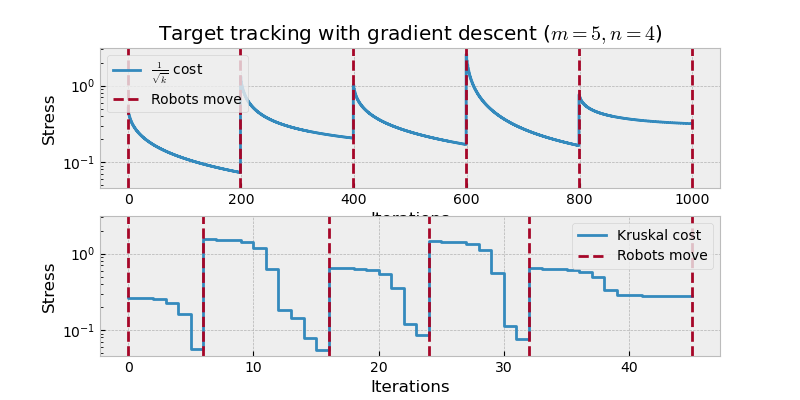
\includegraphics[width=\textwidth,trim=50 0 50 10, clip]{kruskal_5_4.png}
%         \caption{Smaller tracking example with $n=4$ robots and $m=5$ measurements}
%     \end{subfigure}
%     \begin{subfigure}{\linewidth}
%         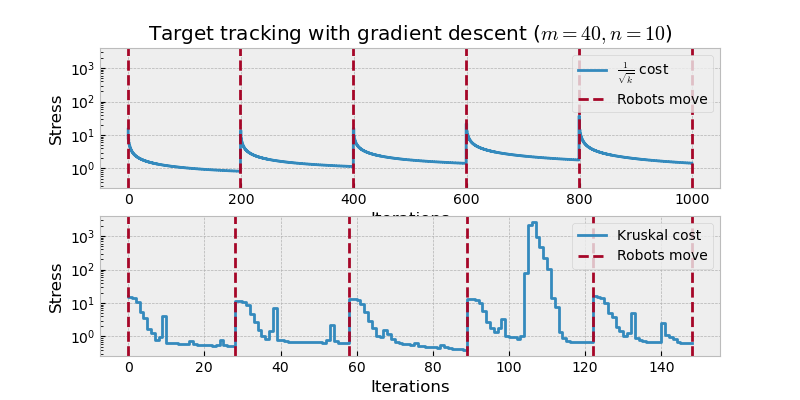
\includegraphics[width=\textwidth,trim=50 0 50 10, clip]{kruskal_40_10.png}
%         \caption{Larger tracking example with $n=10$ robots and $m=40$ measurements}
%     \end{subfigure}
%     \caption{Two different cases of robot tracking. } \label{fig:kruskal}
% \end{figure}
\begin{figure}[ht]
    \centering
    \includesvg[width=\linewidth]{kruskal.svg}
    \caption{Comparison of convergence speeds for the different algorithms.}
    \label{fig:kruskal}
\end{figure}
The plots above cover a range of reasonable values for $n$ and $m$. For values larger than this, the Riemannian elevator takes too much time and memory to run. While the difference in speed is not large, it should be noted that Kruskal's algorithm requires virtually no tuning, while the other two step schedules required tuning to achieve good performance. Nonetheless, it is not a large improvement and is not key to the success of the tracking algorithm. 

In figures~\ref{fig:point-est-small} and~\ref{fig:point-est-large}, the point estimation from distance measurements is showcased. A number of points were generated with noisy distance measurements between them. These values were passed to the Riemannian elevator which generated an initial estimate of the positions, which were further refined by Kruskal's gradient descent method.
\begin{figure}[ht]
    \centering
    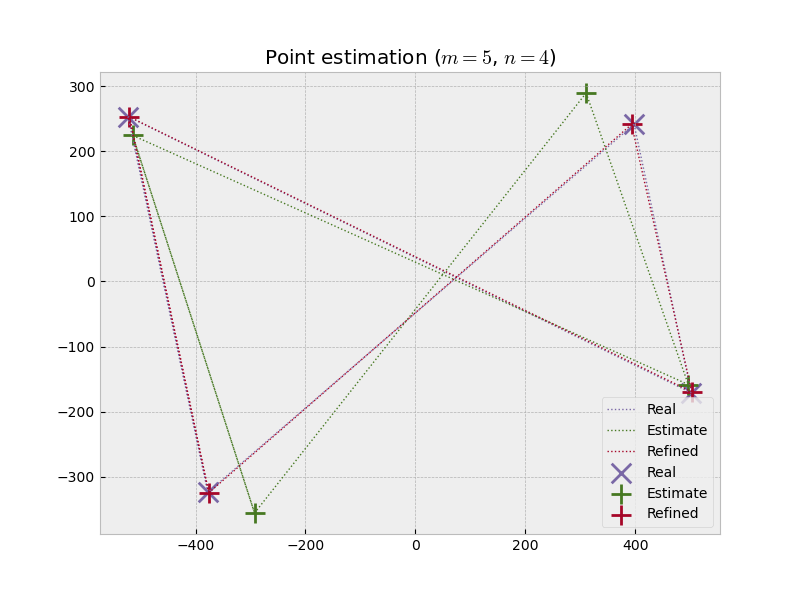
\includegraphics[width=\linewidth,trim=0 20 0 30, clip]{point_est_5_4.png}
    \caption{A smaller example of point estimation.}
    \label{fig:point-est-small}
\end{figure}
\begin{figure}[ht]
    \centering
    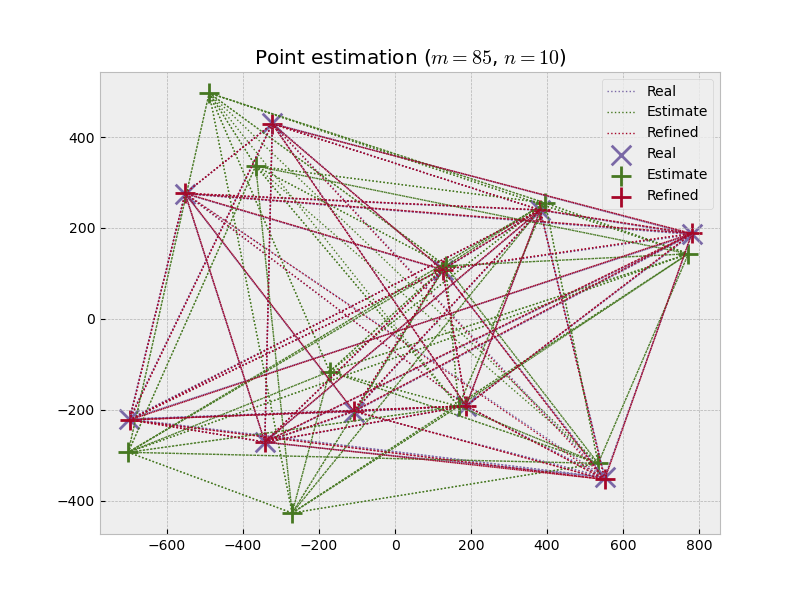
\includegraphics[width=\linewidth,trim=0 20 0 30, clip]{point_est_85_10.png}
    \caption{A larger example of point estimation.}
    \label{fig:point-est-large}
\end{figure}
% \begin{figure}[ht]
%     \centering
%     \begin{subfigure}{\linewidth}
%         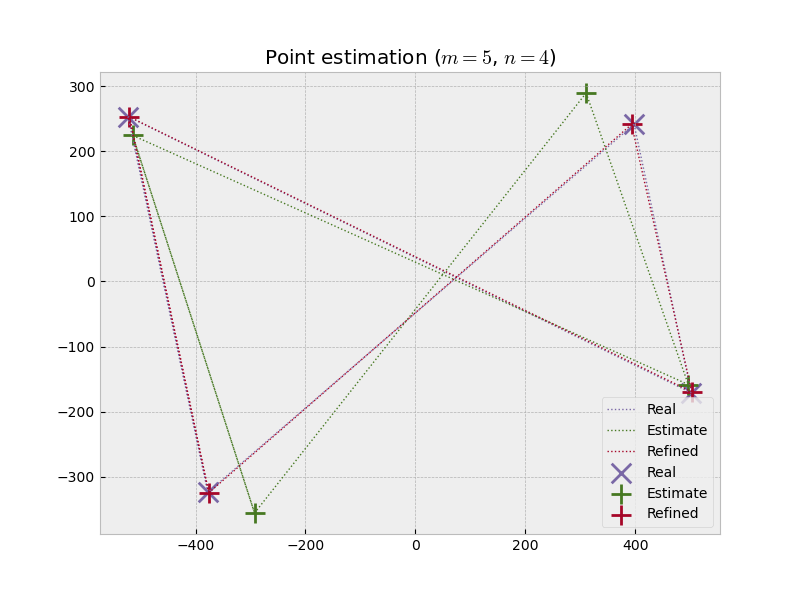
\includegraphics[width=\textwidth,trim=0 20 0 30, clip]{point_est_5_4.png}
%         \caption{A smaller example of position estimation}
%     \end{subfigure}
%     \begin{subfigure}{\linewidth}
%         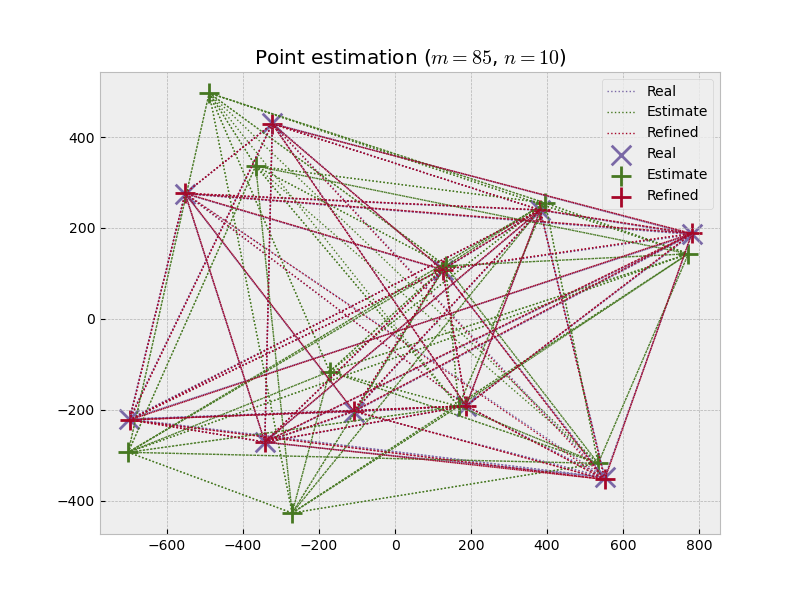
\includegraphics[width=\textwidth,trim=0 20 0 30, clip]{point_est_85_10.png}
%         \caption{A larger example of position estimation}
%     \end{subfigure}
%     \caption{Position estimation from only distance measurements. While there is ambiguity in the rotation and positions of the estimates, they have been rotated and translated to align with the true value for clarity.} \label{fig:riemann}
% \end{figure}
Further, in figure~\ref{fig:RE-accuracy}, we see the overall accuracy performance of the combined Riemannian elevator and gradient descent. For a graph with a given number of vertices $n$, the number of ways to connect two of the vertices with a directed edge is given by 
\begin{align}
    P(n, 2) = \frac{n!}{(n-2)!} = n (n-1)
\end{align}
Therefore, we can determine experimentally that at fewer vertices, $50\%$ accuracy is achieved when around $50\%$ of the possible edges are utilized. As the number of vertices grows, the number of required edges for $50\%$ accuracy shrinks down to about $30\%$. While this is in no way conclusive, and obviously dependant on the level of noise, it does show the power of the Riemannian elevator. 
\begin{figure}[ht]
    \centering
    \includesvg[width=\linewidth]{RE_accuracy.svg}
    \caption{These plots show the success rate of the Riemannian elevator to provide an initial point for which the subsequent gradient descent step converges to the correct arrangement of vertices.}
    \label{fig:RE-accuracy}
\end{figure}

Finally, below in figures~\ref{fig:multi-track} and~\ref{fig:single-track} are some plots of the complete tracking pipeline. It is clear that, while the system is capable of tracking positions with noisy incomplete measurements, the orientation tracking performance degrades and eventually diverges with larger noise. 
\begin{figure*}
    \begin{subfigure}{0.49\linewidth}
        \includesvg[width=\linewidth]{m45_n10_s0.svg}
        \caption{$n=10, m=45$. No noise.}
        \label{fig:track-partial-noiseless}
    \end{subfigure}
    \hfill
    \begin{subfigure}{0.49\linewidth}
        \includesvg[width=\linewidth]{m45_n10_s200.svg}
        \caption{$n=10, m=45$. Large noise.}
        \label{fig:track-partial-noisy}
    \end{subfigure}
    \begin{subfigure}{0.49\linewidth}
        \includesvg[width=\linewidth]{m90_n10_s0.svg}
        \caption{$n=10, m=90$. No noise.}
    \end{subfigure}
    \hfill
    \begin{subfigure}{0.49\linewidth}
        \includesvg[width=\linewidth]{m90_n10_s200.svg}
        \caption{$n=10, m=90$. Large noise.}
    \end{subfigure}
    \caption{Sample tracking performance for $n=10$ robots with varying numbers of measurements and noise. Dashed line is ground truth, red line is estimated state.}
    \label{fig:multi-track}
\end{figure*}
\FloatBarrier
\begin{figure}[ht]
    \centering
    \includesvg[width=\linewidth]{m120_n15_s300.svg}
    \caption{Tracking $n=15$ robots with $m=120$ measurements, e.g. $57\%$ connectivity, with very large noise.}
    \label{fig:single-track}
\end{figure}